\documentclass[12pt,a4paper,titlepage,oneside,BCOR1cm]{scrreprt}



\usepackage[utf8]{inputenc}
\usepackage{graphicx}
\graphicspath{ {images/} } 
\usepackage[final]{pdfpages}
\usepackage{fancyhdr}
\usepackage[pdfpagelabels]{hyperref}
\usepackage{amsmath,amstext,amssymb}
\usepackage{rotating}
\usepackage{afterpage}

\usepackage[english,german]{babel}
\usepackage{csquotes}

\usepackage[style=alphabetic,sorting=nty,backend=bibtex]{biblatex}
\addbibresource{bibliography.bib}

%\bibliographystyle{gerunsrt} % Literaturangaben nach Auftreten sortieren %{gerplain}

\date{\today}
\author{Robin Maximilian Ruth}
\title{Bachelorthesis proposal -- Sparked}

\begin{document}
\thispagestyle{empty}

\begin{figure}[htbp]
\centering
 \begin{minipage}[b]{41 mm}
   
\includegraphics[width=40 mm]{./figures/DAI_Logo.png}
 \end{minipage}
\end{figure}

~\vspace{0.5cm}

\begin{center}
\begin{Huge}
Technische Universitaet Berlin\\
\vspace{1mm}
\end{Huge}{\Large Fakultaet IV - Elektrotechnik und Informatik\\
Fachgebiet AOT\\
Prof. Dr. Sahin Albayrak}\\

\vspace{26mm}
\begin{LARGE}
Bachelorthesis proposal\\
\end{LARGE}
\vspace{8mm}
\begin{LARGE}
An intuitive user interface for the automated machine learning project CODA\\
\end{LARGE}
\vspace{3 cm}
Robin Ruth\\
Matrikel--Nummer 316672\\
\vspace{1cm}
\begin{tabular}{lll}
    \textbf{Betreuer} & Researcher Christian Geissler & Dipl.-Inform.\\
\end{tabular}


\end{center}

\tableofcontents
\thispagestyle{empty}


\pagenumbering{arabic}
\chapter{Motivation}
With the ongoing digitalization and the generation of big data in most aspects of society, data driven approaches to every day problems become more and more viable. One way to evaluate these large datasets is with a machine learning approach. Machine learning, though powerful, has its own challenges. Not every machine learning approach is applicable for every problem, not every algorithm will perform in reasonable time on every data, the list goes on.

A lot of intimate knowledge and intuition about machine learning algorithms is needed to select a good approach to a given problem. Knowledge and intuition that is only developed in few experts. Even then, to optimize for a given problem still requires a lot of time, as most of the time the best hyperparameter settings can only be found by trial and error.

To automate this process, DAI-Labor (Distributed Artificial Intelligence) and GT-ARC (German Turkish Advanced Research Center for ICT) have started CODA, a fundamental research project in algorithm selection and hyperparameter optimization. \cite{CODA-Steckbrief}

This project creates an interface to the CODA project, allowing machine learning enthusiasts and specialists to use the developed solutions and giving the team an interface to demonstrate CODAs capabilities.

The provided user interface may be used in demonstrations as well as by persons with a background in machine learning. The focus is set on a clean workflow, good user guidance and a visual appealing display.




\chapter{Objective}
The overall objective of Sparked is to create a web application and a supporting backend to interface with the CODA backend. 

To develop Sparked an architecture has to be chosen. This includes which languages and technologies will be used in the development process. 

\section{Architecture}

The architecture has to support several use cases:
\begin{itemize}
  \item Demonstration startup
  
  It should be easy to spin up a clean Sparked instance with empty databases for demonstration purposes. Sensible defaults should apply, to make such an instance immediately usable even by an untrained individual.

  \item Configurability

  Changing the CODA Backend should be possible without recompile.

  \item Docker deployment

  Sparked has to run in docker containers on a linux system.

\end{itemize}

Some common characteristics of web applications are not relevant in this project:
\begin{itemize}
  \item User accounts

  All Users will operate on the same data. There will not be any user accounts. Any data uploaded to Sparked is visible to all other users.
  \item Login

  The UI will be open and not contain any login features or any other form of access control.
\end{itemize}

Coda will run on a separate machine, connected via a Kafka bus system. Kafka access is not part of the Sparked project. An encapsulation library written in Java will be provided.

\section{Workflows}

Sparked contains several workflows:
\begin{itemize}
  \item Order creation

  An order can be created. This includes the selection of all values needed to create an order, classifier, metric, test dataset and validation method with their respective parameters.

  After an order is created, it will be split in tasks and put into a queue for processing. This includes persisting them to have a keep them in data on restart.

  \item Test data

  While creating an order, the user may select from a pool of test data but may also chose to upload their own sets. Uploaded files have to be redirected to CODA to allow usage in the evaluation process.

  The data will not be validated in Sparked. Correctly formatted data will be assumed.

  \item Order overview

  View all orders, with their tasks and allows them to be paused or continued if not finished. A Sparked instance will connect to a single backend. 

  \item Order evaluation
  
  Display an evaluation page for order and task results.
\end{itemize}

It is not possible to access multiple CODA backends at the same time. 

Sparked does not contain any evaluation logic or machine learning support itself. As such it is dependent on the data returned from CODA via Kafka. Neither does it contain an error logic. If an error occurs in CODA, Sparked will not provide help. Additionally Sparked will assume correct configuration and service setup. 

\section{Evaluation}

To evaluate the usability and user interface decisions, a think-aloud interview will be conducted. This method helps to understand the expectations a user has at a given point in a workflow and shows if the user is able to use the application in a successful manner without prior knowledge of the program or if help is needed.

The results of the think aloud interview will be discussed in this thesis, but not influence the actual development. Ideally a think aloud interview would be followed by a secondary development block to address the found factors. Instead the results will be collected for possible future projects.

The think aloud interview is not supposed to be a statistical evaluation, the number of participants does not have to be statistically significant. 

\chapter{Work packages}

The project is roughly separated in 3 parts:
\begin{itemize}
  \item Architecture
  \item Development
  \item Evaluation
\end{itemize}


\section{Architecture}
\begin{itemize}
  \item UX Design
  \item UI Design
  \item Technology evaluations
  
  \begin{itemize}
    \item Database
    \item Backend language and technologies
    \item Frontend language and technologies
    \item Frontend chart library
  \end{itemize}  
  \item System architecture
  \item Evaluating similar programs

\end{itemize}  

\section{Development}
\begin{itemize}
  \item Basic setup
  \item Order creation
  \item Data persistence: Database access module
  \item Basic user interface
  \item Test data upload
  \item Order overview page
  \item Integrating Kafka access library / CODA connection
  \item Configuration page
  \item Order evaluation
  \item UI optimization  
  \item Bug fixing
  \item Docker setup
  \item Final deployment on DAI server
\end{itemize}
\section{Think aloud interviews}
  \begin{itemize}
    \item Find test group
    \item Create interview questionnaire
    \item Hold the interview
    \item Evaluate the statements
  \end{itemize}

\chapter{Schedule}

\hspace*{-1.5in}
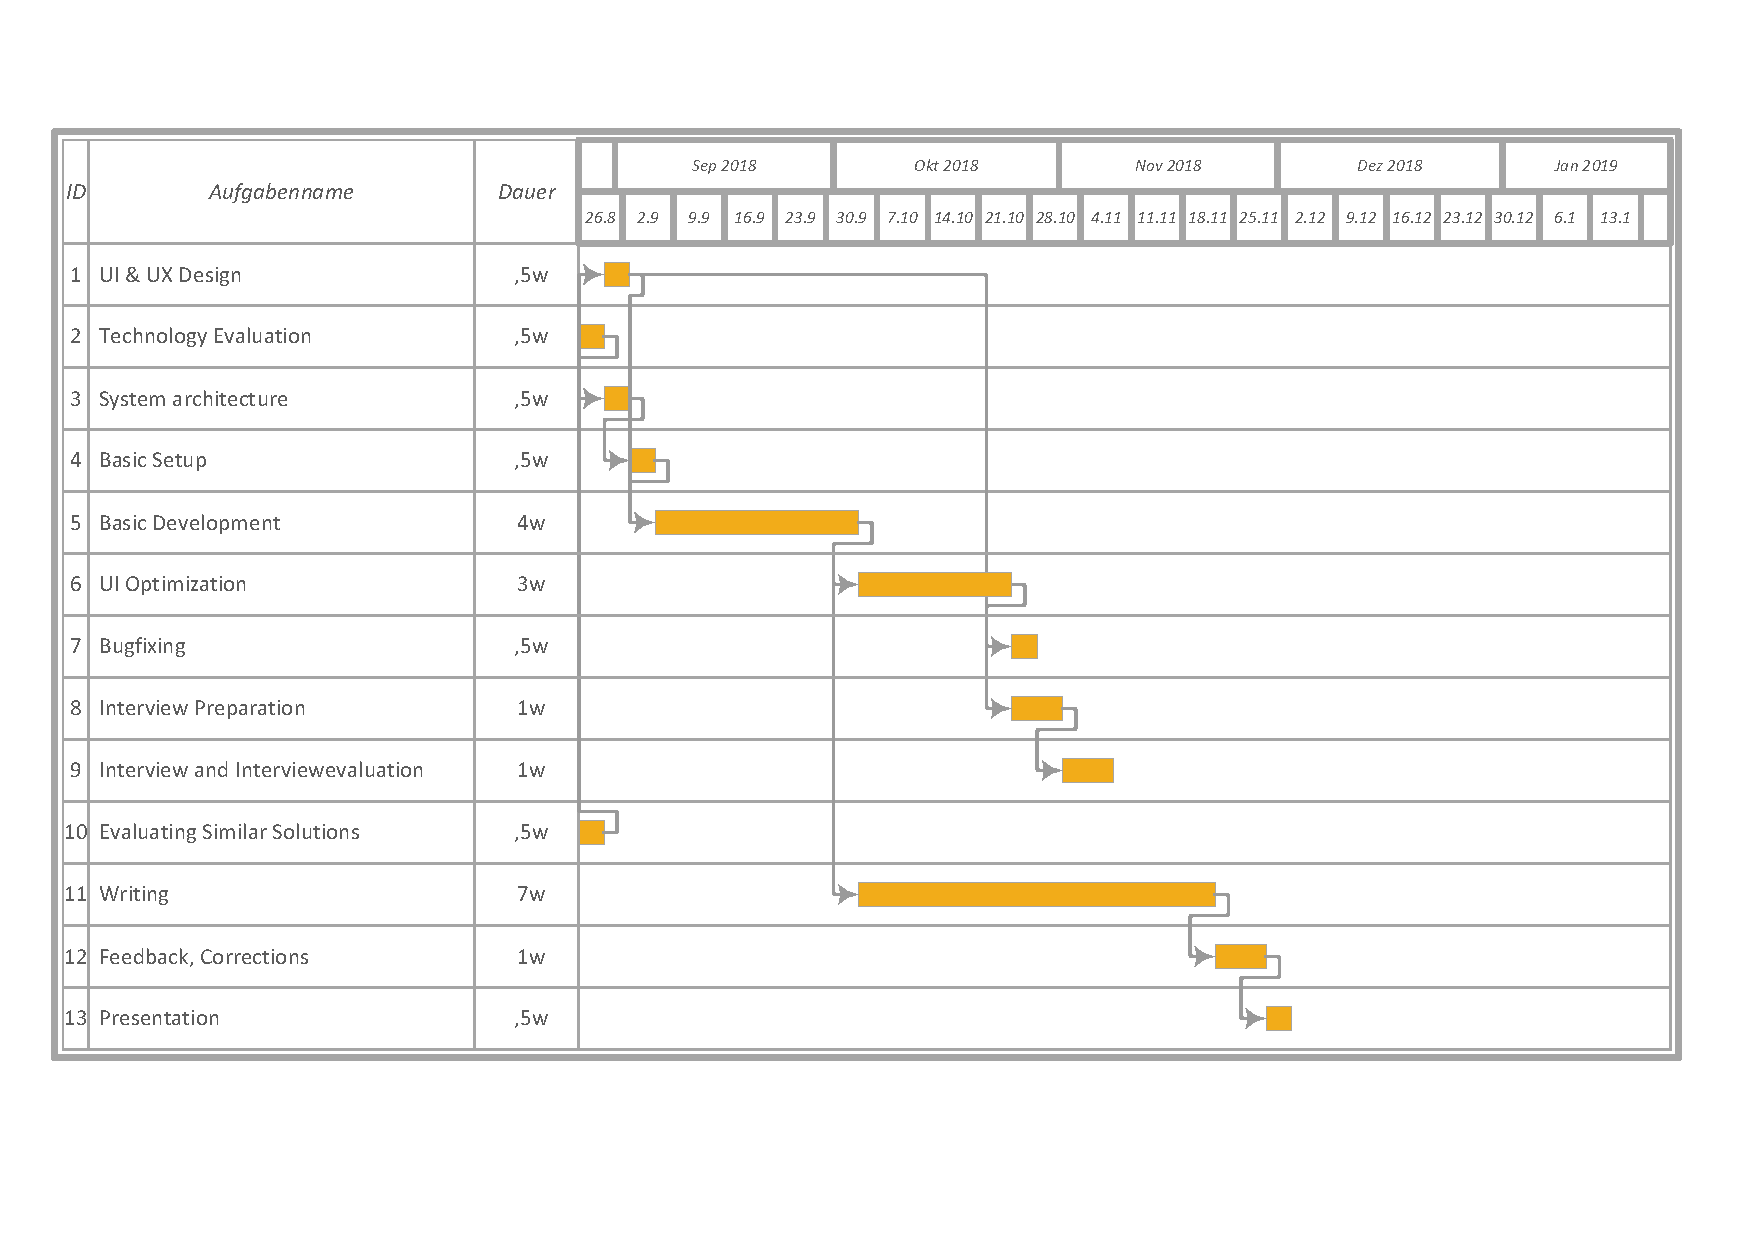
\includegraphics[width=\paperwidth]{gantt-proposal-3.pdf}

\chapter{Organizational}
\begin{itemize}
\item Language of this Bachelor thesis is english.
\item The thesis will be written with pdflatex.
\item Choosing programming languages and technologies are not defined and part of the development process.
\item Supervisors is Christian Geißler
\item Evaluators are Prof. Dr. Albayrak and Prof. Kao
\end{itemize}

\chapter{Appendix}
\newpage

\nocite{*}

\printbibliography

\end{document}
